%=========================================================================
% (c) Michal Bidlo, Bohuslav Křena, 2008

%\usepackage{xcolor}
\newcommand\note[1]{{\Large \textcolor{red}{#1}}}

\chapter{Úvod}
Počítačové sítě, zejména Internet, v dnešním světě zaujímají jednu z nejvýznamnějších rolí. Počínaje výzkumem a vědeckými experimenty, konče běžným životem většiny lidí. Jen za posledních deset let se počet uživatelů Internetu více než ztrojnásobil z cca jedné miliardy lidí na tři miliardy. Počítačové sítě propujují celý svět a jsou neustále rozšiřovány, vylepšovány a modernizovány. To vede k větším nárokům na použité technologie a zdroje. 

Avšak se zvyšujícím počtem uživatelů roste i počet útoků na různé počítačové sítě, kterými se útočníci snaží získat informace či poškodit oběť. Síťový útok\cite{rfcAttack} je definován jako záměrný akt, kde se entita snaží překonat bezpečnostní služby a porušit bezpečnost systému. Vznikají tím pádem systémy na detekci takovýchto útoků, aby správcí sítí dokázali reagovat na vzniklou situaci.

Jeden z těchto systémů vznikl ve sdružení CESNET s názvem NEMEA (Network Measurements Analysis). Tento systém analyzuje síťový provoz a zaznamenává podezřelé toky jako agregované události do databáze. Na větší síti (stovky až tisíce připojených zařízení) je takovýchto událostí vytvořeno až několik tisíc denně. S tím nastává problém jak dané události jednoduše analyzovat a rozpoznat na jaké události se zaměřit a na které nebrát zřetel.

Pro efektivní analýzu velkého množství dat je nejvhodnější vizualizace dle vhodných metrik. Cílem této bakalářské práce je vytvořit aplikaci pro vizuální analýzu bezpečnostních událostí na síti monitorované systémem Nemea. 

Důležitým aspektem vytvořené aplikace je důraz na použití moderních knihoven podporující tvorbu dynamických webových aplikací, které jsou dostupné na různých typech zařízeních. Společně s tím je kladen důraz na uživatelskou přívětivost a jednoduchost prostředí, ve kterém bude probíhat vizuální analýza událostí.

Celou aplikaci navíc bude možno libovolně přizpůsobit tak, aby vyhovovala potřebám daného správce sítě. V aplikaci bude zavedena technika {\it drill-down}, která napomáhá rychlé a přehledné analýze velkého množství dat bez ztráty informací o analyzované události. Drill-down spočívá v postupném zvyšování rozlišení dat, která analyzujeme a postupujeme směřem shora dolů.

Aplikace bude pracovat s konkrétním formátem dat nazvaný IDEA. Tento formát dat je specifikován sdružením CESNET a slouží jako prostředek pro sdílení dat bezpečnostních událostí mezi různými systémy. Díky tomu lze systém kdykoliv přenést na jiný zdroj databáze než je systém Nemea, např. v rámci sdružení CESNET na systém Warden nebo Mentat.

Aplikace bude integrována do současného NEMEA systému pod názvem Nemea Dashboard a bude s ním společně distribuována jako front~end celého systému.

\chapter{Monitoring sítě}

V rozlehlejších sítích jako např. páteřní či firemní síť je téměř nutností monitorovat a analyzovat provoz na síti, abychom byli informování o jejím aktuálním stavu, vytížení a zejména negativních vlivech na monitorovanou síť.

Monitoring lze rozdělit do dvou částí. Aktivní a pasivní způsob.

\section{Nemea}

Network Measurements Analysis, zkráceně Nemea, je systém, který dovoluje seskládat celek pro automatizovanou analýzu toků získaných ze síťového monitoringu v reálném čase. Systém se skládá z oddělených stavebních bloků nazývané moduly. Tyto jednotlivé moduly jsou následně propojeny pomocí rozhraní.

Moduly jsou nezávislé pracovní jednotky, které obecně přijímají proud dat na svých vstupech, zpracují či zanalyzují daná data a následně je odešlou ze svých výstupních rozhraní jako proud dat pro další moduly. Modul může například tvořit statistiky o přijatých datech a na základě těchto statistik detekovat určité typy síťového útoku. Detekovaný útok je popsán datovým záznamem, který je odeslán přes výstupní rozhraní dalším modulům, které s daným záznamem dále pracují, např. jej uloží v IDEA formátu (viz sekce \ref{sec:idea}) do databáze nebo ze získaných statistik dokáží detekovat anomálie v síťovém provozu a dokáží tak jednotlivé pokusy od jednoho útočníka agregovat a zpracovat jej jako jediný útok skládající se z několika desítek až stovek pokusů o útok, které odděleně nemají význam a administrátor sítě by je snadno přehlédl nebo ignoroval.

Jednotlivé moduly nemají osamoceně velký význam, ale pokud tyto moduly spojíme ve složitější systém, získáme komplexní nástroj na aktivní analýzu síťových dat schopný detekovat a identifikovat útoky na monitorovanou síť, který následně detekované útoky uloží do databáze a webová aplikace, kterou v této práci navrhujeme, uložené útoky zobrazí.

Nemea je také schopná přístupu ``store-and-ex-post'', který lze vidět na obrázku \ref{fig:nemea-schema}. Jsou zde dva moduly spojené jedním rozhraním. První modul čte záznamy toků ze souboru a druhý modul počítá statistiky těchto přečtených toků. Tento přístup je charakteristický tím jak nakládá se síťovými daty. Ty prvně uloží a až poté začíná systém s analýzou síťových dat. Oproti streamovému zpracování síťových dat je tento systém náročnější na datový prostor, ale analýza \note{(najít proč je lepší)}
\begin{figure}[ht]
  \centering
    
\includegraphics[width=0.5\textwidth]{fig/nemea-basic.pdf}
  \caption{Minimální příklad Nemea systému obsahující pouze dva moduly.} \label{fig:nemea-schema}
  
\end{figure}

Z takto základních bloků lze postavit i velmi komplexní systém jak je vidět na obrázku \ref{fig:nemea-example-2}, kde jsou data přijímána v reálném čase z IPFIX\cite{ipfix} kolektoru. Data jsou předzpracována, analyzována několika algoritmy a následně jsou vytvořeny události, které jsou nahlášeny. Každá z těchto úloh je jeden modul, který může být znovu použitý na několika různých místech. Tím se šetří zdroje a nároky na tvorbu modulů.

\begin{figure}
  \centering
    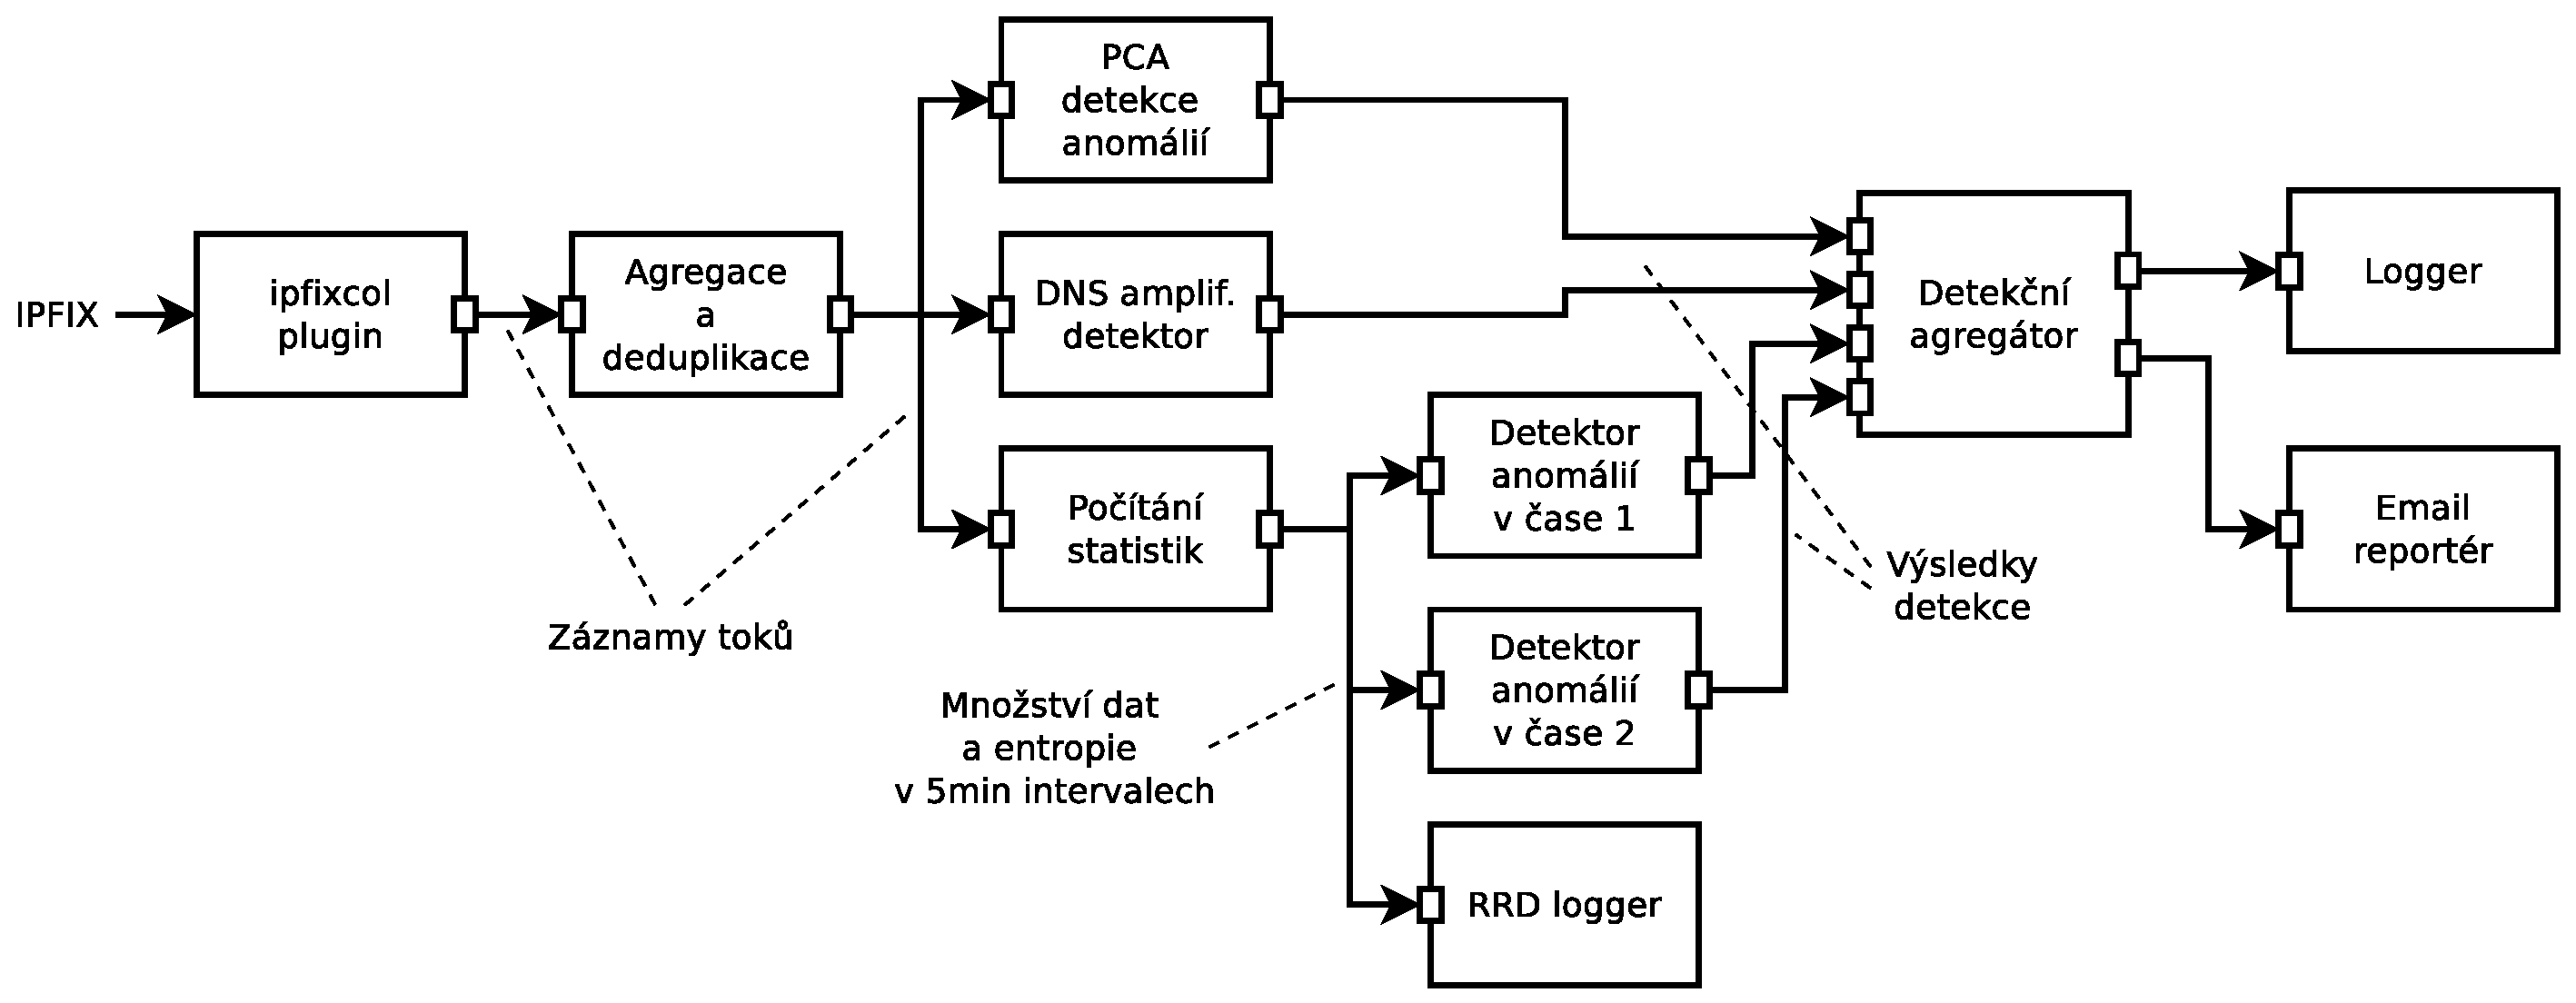
\includegraphics[width=1\textwidth]{fig/nemea-example-2-cz.eps}
  \caption{Komplexní příklad Nemea systému, který kolektuje data, předzpracovává je, provádí detekci anomálií a útoků a následně detekované události ukládá a reportuje.} \label{fig:nemea-example-2}
  
\end{figure}


%\subsection*{Hlavní komponenty}

\subsection{Modul}

Každý modul je samostatný program nezávislý na ostatních. To sice zvyšuje nároky na systém, ale dovoluje větší variabilitu při návrhu modulu. Ten je, díky tomuto návrhu, možno naprogramovat v libovolném jazyce, sledovat a řídit spotřebu zdrojů každého modulu zvlášť a zejména v případě nefungujícího modulu se celý systém Nemea dokáže zotavit z chyby naprosto bez problémů. Modulární systém navíc dovoluje přidávat a odebírat jednotlivé moduly za běhu, což je v produkčním prostředí jedna ze základních vlastnostní kvalitního monitorovacího systému.

Při zapojení a startu nového modulu se modul periodicky snaží připojit na definované rozhraní. Pokusy o spojení jsou sledovány Nemea Supervisorem, kterým lze spravovat všechny moduly v systému a pokud se modulu nepodaří po několika pokusech připojit na rozhraní, je modul ukončen.

\subsection{Rozhraní}

Všechny rozhraní jsou výhradně jednocestná a přenos dat je realizován formou jednotlivých záznamů. Všechny záznamy poslané přes jedno konkrétní rozhraní mají vždy stejný formát, nicméně mezi rozhraními se formát může lišit. 

Protokol pro dynamickou tvorbu formátu je nazván UniRec. Ten specifikuje nejen formát záznamu, ale také jak záznam vytvořit a jak zpracovat.

Pro tvorbu rozhraní je vytvořena sdílená knihovna libtrap, která využívá Traffic Analysis Platform (zkráceně TRAP) pro komunikaci mezi různými rozhraními.

\subsubsection{UniRec}

\section{IDEA}
\label{sec:idea}

Pro potřebu sdílení informací o síťových událostech mezi různými skupinami a zařízeními (např. honeypoty, analyzéry systémových zpráv, analyzéry provozu na síti, netflow sondy a další) existuje několik formátů záznamu takovéto události. Nicméně žádný z nich není natolik univerzální, aby byl vždy a všude použitelný a pokud se k takovému formátu blíží, tak není natolik detailní, aby pokryl většinu důležitých informací.

IDEA, neboli Intrusion Detection Extensible Alert, je formát záznamu síťové události specifikovaný sdružením CESNET. IDEA si klade za cíl specifikovat takový formát záznamu, který je univerzální, přenositelný, ale zároveň dost konkrétní a snadno pochopitelný bez rozsáhlé dokumentace k jednotlivým polím.

Vzorový záznam generovaný systémem Nemea je vyobrazený níže. Jak je vidět, formát je spefikovaný jako JSON dokument. 

\begin{lstlisting}[
    language=Python,
    caption=My caption here,
    label=code1,
    showspaces=false,                % show spaces everywhere adding particular underscores; it overrides 'showstringspaces'
    showstringspaces=false,          % underline spaces within strings only
    showtabs=false]
{
    "ID" : "73e0b136-aeb8-4aae-bb80-9bfb4f258847",
    "Target":[{
        "Proto":["udp","dns"],
        "IP4":["10.0.0.135"],
        "InPacketCount":393
    }],
    "PacketCount":393,
    "Type":["Flow","Statistical"],
    "CeaseTime":"2016-04-07T22:34:38Z",
    "ByteCount":453129,
    "FlowCount":131,
    "Category":["Availibility.DDoS"],
    "CreateTime":"2016-04-07T22:34:52Z",
    "Node":[{
            "SW":["Nemea","amplification_detection"],
            "Name":"cz.cesnet.nemea.amplification_detection"
    }],
    "EventTime":"2016-04-07T22:19:25Z",
    "Source":[{
            "IP4":["192.1.0.201"],
            "Proto":["udp","dns"],
            "OutPacketCount":393,
            "InPacketCount":767
        }],
    "Format":"IDEA0",
    "Description":"DNS amplification",
    "DetectTime":"2016-04-07T22:34:38Z"
}
\end{lstlisting}

\label{Vzorový IDEA záznam z Nemea systému. Některé části byly vynechány nebo zkráceny.}

\section{Další monitorovací systémy}

Na trhu jsou v současné době různá dostupná řešení pro detekci a vizualizaci síťových bezpečnostních událostí, nicméně valná hromada z nich je komerční a hlavně vázaná na konkrétní hardware od daného výrobce. Klient tudíž většinou nekupuje software, ale hardware s přiloženým software. 

\chapter{Technologie}
\section{Dostupné technologie}
\section{Výběr technologií}
\section{Zvolené technologie}

\chapter{Architektura aplikace}
\section{Případy užití}
\section{REST API}
\section{Databáze událostí}
\section{GUI}

\chapter{Implementace}
\section{Backend}
\section{Frontend}
\section{Zabezpečení}
\section{Distribuce}

\chapter{Dosažené výsledky}
\section{Názory uživatelů}
\section{Nasazení v praxi}

\chapter{Závěr}
Závěrečná kapitola obsahuje zhodnocení dosažených výsledků se zvlášť vyznačeným vlastním přínosem studenta. Povinně se zde objeví i zhodnocení z pohledu dalšího vývoje projektu, student uvede náměty vycházející ze zkušeností s řešeným projektem a uvede rovněž návaznosti na právě dokončené projekty.

%=========================================================================
